\documentclass[twoside,a4paper,CCT]{cctart}   % 这是Li Dongfeng改的文件头
\usepackage{amsmath,amsthm,vatola,makeidx,amssymb,amscd,headrule}     % 这是Li Dongfeng改的文件头
\usepackage{amsfonts}                     % 这是Li Dongfeng改的文件头
%\documentstyle[twoside,headrule,vatola]{carticle} %这是原来的文件头
%\input amssym.def
\usepackage{graphicx}                              %这是原来的文件头
\usepackage{epsf}
\usepackage[top=1in,bottom=1in,left=1.25in,right=1.25in]{geometry}
\usepackage{amsmath}
%\usepackage{tikz}
\usepackage{amsmath,amssymb}
\usepackage{tikz}
\input scrload.tex    %调用花体字: {\scr A,B,C,...}
%--------------------------Page Format--------------------------
\headsep 0.2 true cm \topmargin 0pt \oddsidemargin 0pt \footskip
2mm \evensidemargin 0pt \textheight 21 true cm \textwidth 14.7
true cm \setcounter{page}{1}
%\parskip 0.2cm
\parindent 2\ccwd
\nofiles
%---------------------------------------------------------------
\def\sec#1{
\vskip.12in \noindent{\Large\bf\zihao{-4}\heiti #1} \vskip.1in}
\def\subsec#1{
\vskip.1in \flushpar{\zihao{5}\heiti #1} \vskip.1in}
\def\de#1{{\heiti\bf #1}\quad}
\begin{document}
\TagsOnRight \abovedisplayskip=10.0pt plus 2.0pt minus 2.0pt
\belowdisplayskip=10.0pt plus 2.0pt minus 2.0pt
%====================================================================
%\catcode`@=11 \long\def\@makefntext#1{\parindent 1em\noindent
%\hbox to 0pt{\hss$^{}$}#1} \catcode`\@=12
%====================================================================

\renewcommand{\baselinestretch}{1.0}


\newfont{\htxt}{eufm10 scaled \magstep0}
%\newfam\euffam
\font\tenthxt=eufm10 scaled \magstep0 \font\tenBbb=msbm10 scaled
\magstep0 \font\tencyr=wncyr10 scaled \magstep0 \font\tenrm=cmr10
scaled \magstep0 \font\tenbf=cmb10 scaled \magstep0


\def\cyr{\tencyr}




\renewcommand{\proofname}{\bf 证明}
\newtheorem{lemma}{引理}[section]
\newtheorem{guess}{猜测}[section]
\newtheorem{define}{定义}[section]
\newtheorem{theorem}{定理}[section]
%-----------------------作者定义


%-----------------------作者定义结束
\def\binom#1#2{{#1\choose#2}}
\def\qed{\hfill\raisebox{0.1truecm}{\framebox[0.2truecm]{\ } } }
\def\su{\mathop{\sum}\limits}
\def\Cal#1{ {\cal #1 \rm}  }
%---------------------------------------------------------------
\def\evenhead{{\protect\small{\zihao{-5}\songti \hfill \qquad\qquad
\qquad} \hfill {\zihao{-5}\songti }}}
\def\oddhead{{\protect\small {\zihao{-5}\songti }
\hfill {\small\zihao{-5}\songti }\hfill}}
%---------------------------------------------------------------

\vspace*{-13mm}

\thispagestyle{empty}

%%%%%%%%%%%%%%%%%%%%%%%%%%%%%%%%%%%%%%%%%%%%%%%%%%%%%%%%%%%%%%%%%


\ziju{0.025} \vspace*{.26in}

\centerline{\huge $1\times 4$长方块覆盖方形栅格的计数表示} \vskip .1in

%-------------------------------------------------------------------------

 %\footnotetext{基金项目: 国家自然科学基金资助课题(No. 10271026),
%福建省自然科学基金资助项目(No. F0310010).}

\footnotetext{E-mail: $*$ huih1984@163.com}

%-------------------------------------------------------------------------

\centerline{\fangsong\large\zihao{4} 惠慧$^{1}$ } \vskip.12in


%\centerline{\small\zihao{-5}(1.南京大学数学系,南京,江苏, 210093)}

\vskip.25in
{\narrower\fangsong\zihao{-5}\small {\zihao{-5}\heiti 摘要:}\ \
在文章$Kasteleyn^{[1]}$ 中,$Kasteleyn$($Fisher$和$Temperley$ 同时独立)开创性研究了$1 \times 2$长方块在栅格上的覆盖数计算问题。那么如果是$1 \times 3$长方块或者$1 \times 4$长方块甚至更多,结果又是怎样的呢?文章不打算讨论$1 \times 3$ 长方块,而直接讨论$1 \times 4$ 长方块的情况,因为在4的情况下,计数表达方法存在一个显而易见的推广,从而让问题的研究更集中在延拓后的性质探讨和计算上, 在3 的情形却没有。更进一步的看,$1 \times (2n)$的长方块的覆盖问题都可以得到延拓,出于聚焦计算问题的需要,这里只讨论$1\times 4$的情形。文章对内维数为2 的情形$det(A)=pfaffian^{2}(A)$ 的结果做了推广,得出本文的一个关键结果即在内维数为4 的情况下,延拓矩阵、行列式以及$pfaffian$ 定义,得到 $det(A)=pfaffian^{4}(A)$。从形式上看,这个结果相当有趣!但是计算问题却变的非常的不显然,与一般矩阵作类比,得到一些此类矩阵的结果作为文章的结尾。

{\zihao{-5}\heiti\tenbf 关键词:}\ \ 双重维数矩阵; 内维数; 多米诺覆盖; 外积; $pfaffian$;

%{\tenbf\zihao{-5}\heiti MR(2000) 主题分类:}\ \ 54C10; 54D55 /
%{\tenbf\zihao{-5}\heiti 中图分类号:} O189.1
 }

\normalsize

\baselineskip 15pt \vskip.15in

\sec{0 引言}
关于$dimer$覆盖数的计算问题,起源于$Kasteleyn^{[1]}$的文章,文章给出了$dimer$在$m \times n$的块状上和环面上的覆盖数的计算公式。但是用$tetramer$覆盖的公式却没有研究结果,用$1\times n$覆盖的文章有$Mathar^{[4]}$,但是文章只讨论了被覆盖为$9 \times n$的计算公式,本文讨则关注一般性的计算问题。
%数学公式在推广到更高阶的情形,情况往往变得复杂,比如方程解的问题,在小于五次时,有比较简单根式形式,而高于五次的方程一般而言没有根式解,给出深刻的约束条件,高阶方程的根式解依然存在,这个
% 数学历史上的著名问题给人深深的哲思启发。理论的推广几乎总是去除局限的部分,余下的情形就可以拓展开来,发现更多的现象和本质,本文接下来就讨论$1 \times 4$骨牌覆盖数的计算公式。

%很容易得到类似于$pfaffian$的表达形式,进而作者一直在寻找转换成矩阵表达形式,之所以这么做是因为从形式上来看,这种矩阵的存在完全符合数学符号的形式美,经过一番努力,终于找到了相应的矩阵形式。而这种拓展的矩阵形式本身却更有耐人寻味的结构美,作者没有见过有什么文献对这种形式的矩阵有深入的研究,这里作者只得出了一些少量的结果,作者能力有限,希望有更多的研究者参与其中来研究这种矩阵。

\sec{1 表示方法}


\begin{center}
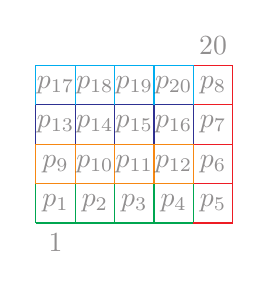
\begin{tikzpicture}[radius=0.1cm]
\selectcolormodel{cmyk}

\node[opacity=0.5] at (.25,-.25) {$1$};
\draw[green, step=.5] (0,0)grid(2,.5);
\node[opacity=0.5] at (.25,.25) {$p_{1}$};
\node[opacity=0.5] at (.75,.25) {$p_{2}$};
\node[opacity=0.5] at (1.25,.25) {$p_{3}$};
\node[opacity=0.5] at (1.75,.25) {$p_{4}$};
\draw[red, step=.5] (2,0)grid(2.5,2);
\node[opacity=0.5] at (2.25,.25) {$p_{5}$};
\node[opacity=0.5] at (2.25,.75) {$p_{6}$};
\node[opacity=0.5] at (2.25,1.25) {$p_{7}$};
\node[opacity=0.5] at (2.25,1.75) {$p_{8}$};
\draw[orange, step=.5] (0,0.5)grid(2,1);
\node[opacity=0.5] at (.25,.75) {$p_{9}$};
\node[opacity=0.5] at (.75,.75) {$p_{10}$};
\node[opacity=0.5] at (1.25,.75) {$p_{11}$};
\node[opacity=0.5] at (1.75,.75) {$p_{12}$};
\draw[blue, step=.5] (0,1)grid(2,1.5);
\node[opacity=0.5] at (.25,1.25) {$p_{13}$};
\node[opacity=0.5] at (.75,1.25) {$p_{14}$};
\node[opacity=0.5] at (1.25,1.25) {$p_{15}$};
\node[opacity=0.5] at (1.75,1.25) {$p_{16}$};
\draw[cyan, step=.5] (0,1.5)grid(2,2);
\node[opacity=0.5] at (.25,1.75) {$p_{17}$};
\node[opacity=0.5] at (.75,1.75) {$p_{18}$};
\node[opacity=0.5] at (1.25,1.75) {$p_{19}$};
\node[opacity=0.5] at (1.75,1.75) {$p_{20}$};
\node[opacity=0.5] at (2.25,2.25) {$20$};
\end{tikzpicture}
\end{center}
采用$Kasteleyn^{[1]}$相同的表示方法,$C=(p_{1},p_{2},p_{3},p_{4})(p_{5},p_{6},p_{7},p_{8})...(p_{N-3},p_{N-2},p_{N-1},p_{N})$.\\
    其中$(p_{j},p_{j+1},p_{j+2},p_{j+3})$为一个长方块的四个连续坐标。

    \begin{equation}\label{1}p_{1}<p_{2}<p_{3}<p_{4},p_{5}<p_{6}<p_{7}<p_{8}
   ,...,p_{N-3}<p_{N-2}<p_{N-1}<p_{N}\end{equation}

   \begin{equation}p_{1}<p_{5}<...<p_{N-3}\end{equation}

   \begin{equation}a_{(i,j;i+1,j;i+2,j;i+3,j)}=1,1\leq i \leq m-3,1\leq j\leq n\end{equation}
   \begin{equation}a_{(i,j;i,j+1;i,j+2;i,j+3)}=1,1\leq i \leq m,1\leq j\leq n-3\end{equation}
   \begin{equation}a_{(i,j;i^{'},j^{'};i^{''},j^{''};i^{'''},j^{'''})}=0,other \end{equation}

   \begin{equation}pfaffian(A_{4})=\sum\limits_{\sigma=p_{1}p_{2}...p_{N}satisfy(1)(2)}sgn\sigma a_{p_{1}p_{2}p_{3}p_{4}}a_{p_{5}p_{6}p_{7}p_{8}}...a_{p_{N-3}p_{N-2}p_{N-1}p_{N}}\end{equation}

   对应的矩阵记为$A_{4}=(a_{ijkl})$,满足$a_{jikl}=-a_{ijkl}$,$i,j,k,l$的任意一个序关系都满足逆序数正负号。
   这样得到的表达式$(6)$,仍然称为$pfaffian$。


\sec{2 $pfaffian \rightarrow det$的转换}

\begin{define}\quad 矩阵的内维数和外维数:
\end{define}
$\begin{bmatrix}
a_{i_{1}i_{2}...i_{n}}\end{bmatrix}_{m}$为$n$个下指标构成的多维矩阵,每个指标取值为$1,2,\cdots,m$,则$n$称为内维数,$m$称为外维数。此文只考虑$n$为4的情形。

\begin{define}\quad 矩阵行列式:
\end{define}

将$[a_{ijkl}]$表示成矩阵的矩阵形式,内部子矩阵的指标为$i,j$,外部矩阵指标为$k,l$,行列式$det$满足如下性质:
\newcounter{Lcount}
\begin{list}{\Roman{Lcount}}
{\usecounter{Lcount}
\setlength{\rightmargin}{\leftmargin}}
%\scriptsize
\item
系数性质,行列式乘以系数k,与在某个指标中的固定取值上乘以k所得矩阵的行列式相等。如取$l=1$如下:
\begin{align*}
s det
  \begin{bmatrix}
  \begin{bmatrix}
  \  a_{1111}&\  a_{2111}&\cdots&\  a_{n111}\\
 \  a_{1211}&\  a_{2211}&\cdots&\  a_{n211}\\
  \cdots&\cdots&\cdots &\cdots& \\
\  a_{1n11}&\  a_{2n11}&\cdots&\  a_{nn11}\\
 \end{bmatrix}
\cdots
\begin{bmatrix}
\  a_{11n1}&\  a_{21n1}&\cdots&\  a_{n1n1}\\
\  a_{12n1}&\  a_{22n1}&\cdots&\  a_{n2n1}\\
  \cdots&\cdots&\cdots &\cdots& \\
\  a_{1nn1}&\  a_{2nn1}&\cdots&\  a_{nnn1}\\
\end{bmatrix}\\
\vdots\\
\begin{bmatrix}
\  a_{111n}& \  a_{211n}&\cdots&\  a_{n11n}\\
\  a_{121n}& \  a_{221n}&\cdots&\  a_{n21n}\\
  \cdots&\cdots&\cdots &\cdots& \\
\  a_{1n1n}& \  a_{2n1n}&\cdots& \  a_{nn1n}\\
\end{bmatrix}
\cdots
\begin{bmatrix}
\  a_{11nn}& \  a_{21nn}&\cdots&\  a_{n1nn}\\
\  a_{12nn}& \  a_{22nn}&\cdots&\  a_{n2nn}\\
  \cdots&\cdots&\cdots &\cdots& \\
\  a_{1nnn}& \  a_{2nnn}&\cdots&\  a_{nnnn}\\
\end{bmatrix}
\end{bmatrix}\\
\\
=det
  \begin{bmatrix}
  \begin{bmatrix}
 sa_{1111}& sa_{2111}&\cdots&sa_{n111}\\
 sa_{1211}& sa_{2211}&\cdots&sa_{n211}\\
  \cdots&\cdots&\cdots &\cdots& \\
sa_{1n11}& sa_{2n11}&\cdots&sa_{nn11}\\
 \end{bmatrix}
\cdots
\begin{bmatrix}
sa_{11n1}& sa_{21n1}&\cdots&sa_{n1n1}\\
sa_{12n1}& sa_{22n1}&\cdots&sa_{n2n1}\\
  \cdots&\cdots&\cdots &\cdots& \\
sa_{1nn1}& sa_{2nn1}&\cdots&sa_{nnn1}\\
\end{bmatrix}\\
\vdots\\
\begin{bmatrix}
\  a_{111n}& \  a_{211n}&\cdots&\  a_{n11n}\\
\  a_{121n}& \  a_{221n}&\cdots&\  a_{n21n}\\
  \cdots&\cdots&\cdots &\cdots& \\
\  a_{1n1n}& \  a_{2n1n}&\cdots&\  a_{nn1n}\\
\end{bmatrix}
\cdots
\begin{bmatrix}
\  a_{11nn}& \  a_{21nn}&\cdots& \  a_{n1nn}\\
\  a_{12nn}& \  a_{22nn}&\cdots&\  a_{n2nn}\\
  \cdots&\cdots&\cdots &\cdots& \\
\  a_{1nnn}& \  a_{2nnn}&\cdots& \  a_{nnnn}\\
\end{bmatrix}
\end{bmatrix}
 \end{align*}
 \item
 符号性质,某个指标下的任意两列交换位置,行列式正负号互换,例如下:
\begin{align*}
det
  \begin{bmatrix}
\vdots\\
 \begin{bmatrix}
 a_{111\xi}& a_{211\xi}&\cdots&a_{n11\xi}\\
 a_{121\xi}& a_{221\xi}&\cdots&a_{n21\xi}\\
  \cdots&\cdots&\cdots &\cdots& \\
a_{1n1\xi}& a_{2n1\xi}&\cdots&a_{nn1\xi}\\
\end{bmatrix}
\cdots
\begin{bmatrix}
  a_{11n\xi}& a_{21n\xi}&\cdots&a_{n1n\xi}\\
  a_{12n\xi}& a_{22n\xi}&\cdots&a_{n2n\xi}\\
  \cdots&\cdots&\cdots &\cdots& \\
 a_{1nn\xi}& a_{2nn\xi}&\cdots&a_{nnn\xi}\\
 \end{bmatrix}\\
\vdots\\
\begin{bmatrix}
  a_{111\eta}& a_{211\eta}&\cdots&a_{n11\eta}\\
  a_{121\eta}& a_{221\eta}&\cdots&a_{n21\eta}\\
  \cdots&\cdots&\cdots &\cdots& \\
   a_{1n1\eta}& a_{2n1\eta}&\cdots&a_{nn1\eta}\\
   \end{bmatrix}
\cdots
\begin{bmatrix}
  a_{11n\eta}& a_{21n\eta}&\cdots&a_{n1n\eta}\\
  a_{12n\eta}& a_{22n\eta}&\cdots&a_{n2n\eta}\\
  \cdots&\cdots&\cdots &\cdots& \\
   a_{1nn\eta }& a_{2nn\eta}&\cdots&a_{nnn\eta}\\
   \end{bmatrix}\\
\vdots\\
    \end{bmatrix}\\
=-det
  \begin{bmatrix}
\vdots\\
 \begin{bmatrix}
   a_{111\eta}& a_{211\eta}&\cdots&a_{n11\eta}\\
   a_{121\eta}& a_{221\eta}&\cdots&a_{n21\eta}\\
  \cdots&\cdots&\cdots &\cdots& \\
   a_{1n1\eta}& a_{2n1\eta}&\cdots&a_{nn1\eta}\\
   \end{bmatrix}
\cdots
\begin{bmatrix}
  a_{11n\eta}& a_{21n\eta}&\cdots&a_{n1n\eta}\\
  a_{12n\eta}& a_{22n\eta}&\cdots&a_{n2n\eta}\\
  \cdots&\cdots&\cdots &\cdots& \\
  a_{1nn\eta }& a_{2nn\eta}&\cdots&a_{nnn\eta}\\
  \end{bmatrix}\\
\vdots\\
 \begin{bmatrix}
   a_{111\xi}& a_{211\xi}&\cdots&a_{n11\xi}\\
   a_{121\xi}& a_{221\xi}&\cdots&a_{n21\xi}\\
  \cdots&\cdots&\cdots &\cdots& \\
a_{1n1\xi}& a_{2n1\xi}&\cdots&a_{nn1\xi}\\
\end{bmatrix}
\cdots
\begin{bmatrix}
  a_{11n\xi}& a_{21n\xi}&\cdots&a_{n1n\xi}\\
  a_{12n\xi}& a_{22n\xi}&\cdots&a_{n2n\xi}\\
  \cdots&\cdots&\cdots &\cdots& \\
  a_{1nn\xi}& a_{2nn\xi}&\cdots&a_{nnn\xi}\\
  \end{bmatrix}\\
\vdots\\
    \end{bmatrix}
\end{align*}
 \item
 加法性质,任意一个列中和式可以分解,例如下
%\begin{align*}
 $$det\begin{bmatrix}
 \begin{bmatrix}\begin{smallmatrix}
 a_{1111} + a_{1111}^{'}& a_{2111} + a_{2111}^{'}&\cdots&a_{n111} + a_{n111}^{'}\\
 a_{1211} + a_{1211}^{'}& a_{2211} + a_{2211}^{'}&\cdots&a_{n211} + a_{n211}^{'}\\
  \cdots&\cdots&\cdots &\cdots& \\
a_{1n11} + a_{1n11}^{'}& a_{2n11} + a_{2n11}^{'}&\cdots&a_{nn11} + a_{nn11}^{'}\\
\end{smallmatrix}\end{bmatrix}
\cdots
\begin{bmatrix}\begin{smallmatrix}
  a_{11n1} + a_{11n1}^{'}& a_{21n1} + a_{21n1}^{'}&\cdots&a_{n1n1} + a_{n1n1}^{'}\\
a_{12n1} + a_{12n1}^{'}& a_{22n1} + a_{22n1}^{'}&\cdots&a_{n2n1} + a_{n2n1}^{'}\\
  \cdots&\cdots&\cdots &\cdots& \\
 a_{1nn1} + a_{1nn1}^{'}& a_{2nn1} + a_{2nn1}^{'}&\cdots&a_{nnn1} + a_{nnn1}^{'}\\
 \end{smallmatrix}\end{bmatrix}\\
\vdots\\
\begin{bmatrix}
  \ \ a_{111n}\ \ \ \ & a_{211n}\ \ \ \ &\cdots&a_{n11n}\\
  \ \ a_{121n}\ \ \ \ & a_{221n}\ \ \ \ &\cdots&a_{n21n}\\
  \cdots&\cdots&\cdots &\cdots& \\
  \ \ a_{1n1n}\ \ \ \ & a_{2n1n}\ \ \ \ &\cdots&a_{nn1n}\\
  \end{bmatrix}
\cdots
\begin{bmatrix}
  \ \ a_{11nn}\ \ \ \ & a_{21nn}\ \ \ \ &\cdots&a_{n1nn}\\
  \ \ a_{12nn}\ \ \ \ & a_{22nn}\ \ \ \ &\cdots&a_{n2nn}\\
  \cdots&\cdots&\cdots &\cdots& \\
   \ \ a_{1nnn}\ \ \ \ & a_{2nnn}\ \ \ \ &\cdots&a_{nnnn}\\
\end{bmatrix}
\end{bmatrix}\\
\\$$
$$=det\begin{bmatrix}
 \begin{bmatrix}
   a_{1111}& a_{2111}&\cdots&a_{n111}\\
   a_{1211}& a_{2211}&\cdots&a_{n211}\\
  \cdots&\cdots&\cdots &\cdots& \\
a_{1n11}& a_{2n11}&\cdots&a_{nn11}\\
\end{bmatrix}
\cdots
\begin{bmatrix}
  a_{11n1}& a_{21n1}&\cdots&a_{n1n1}\\
  a_{12n1}& a_{22n1}&\cdots&a_{n2n1}\\
  \cdots&\cdots&\cdots &\cdots& \\
 a_{1nn1}& a_{2nn1}&\cdots&a_{nnn1}\\
 \end{bmatrix}\\
\vdots\\
\begin{bmatrix}
  a_{111n}& a_{211n}&\cdots&a_{n11n}\\
  a_{121n}& a_{221n}&\cdots&a_{n21n}\\
  \cdots&\cdots&\cdots &\cdots& \\
   a_{1n1n}& a_{2n1n}&\cdots&a_{nn1n}\\
   \end{bmatrix}
\cdots
\begin{bmatrix}
  a_{11nn}& a_{21nn}&\cdots&a_{n1nn}\\
  a_{12nn}& a_{22nn}&\cdots&a_{n2nn}\\
  \cdots&\cdots&\cdots &\cdots& \\
   a_{1nnn}& a_{2nnn}&\cdots&a_{nnnn}\\
   \end{bmatrix}
    \end{bmatrix}
  \\$$
  $$+det
  \begin{bmatrix}
 \begin{bmatrix}
   a_{1111}^{'}& a_{2111}^{'}&\cdots&a_{n111}^{'}\\
   a_{1211}^{'}& a_{2211}^{'}&\cdots&a_{n211}^{'}\\
  \cdots&\cdots&\cdots &\cdots& \\
a_{1n11}^{'}& a_{2n11}^{'}&\cdots&a_{nn11}^{'}\\
\end{bmatrix}
\cdots
\begin{bmatrix}
  a_{11n1}^{'}& a_{21n1}^{'}&\cdots&a_{n1n1}^{'}\\
  a_{12n1}^{'}& a_{22n1}^{'}&\cdots&a_{n2n1}^{'}\\
  \cdots&\cdots&\cdots &\cdots& \\
 a_{1nn1}^{'}& a_{2nn1}^{'}&\cdots&a_{nnn1}^{'}\\
 \end{bmatrix}\\
\vdots\\
\begin{bmatrix}
  a_{111n}& a_{211n}&\cdots&a_{n11n}\\
  a_{121n}& a_{221n}&\cdots&a_{n21n}\\
  \cdots&\cdots&\cdots &\cdots& \\
   a_{1n1n}& a_{2n1n}&\cdots&a_{nn1n}\\
   \end{bmatrix}
\cdots
\begin{bmatrix}
  a_{11nn}& a_{21nn}&\cdots&a_{n1nn}\\
  a_{12nn}& a_{22nn}&\cdots&a_{n2nn}\\
  \cdots&\cdots&\cdots &\cdots& \\
   a_{1nnn}& a_{2nnn}&\cdots&a_{nnnn}\\
   \end{bmatrix}
    \end{bmatrix}\\$$
   % \end{align*}
   \item
   单位元
$$det \begin{bmatrix}
 \begin{bmatrix}
   1& 0&\cdots&0\\
   0& 0&\cdots&0\\
  \cdots& \cdots&\cdots&\cdots \\
0& 0&\cdots&0\\
\end{bmatrix}
\cdots
\begin{bmatrix}
  0& 0&\cdots&0\\
  0& 0&\cdots&0\\
  \cdots& \cdots&\cdots&\cdots \\
 0& 0&\cdots&0\\
 \end{bmatrix}\\
\vdots\\
\begin{bmatrix}
  0& 0&\cdots&0\\
  0& 0&\cdots&0\\
  \cdots& \cdots&\cdots&\cdots \\
   0& 0&\cdots&0\\
   \end{bmatrix}
\cdots
\begin{bmatrix}
  0& 0&\cdots&0\\
  0& 0&\cdots&0\\
  \cdots& \cdots&\cdots&\cdots \\
   0& 0&\cdots&1\\
   \end{bmatrix}
    \end{bmatrix}
    =1$$
      \item
零项元,单位元中的任何内矩阵交换1所在行列到另一个行列,满足存在$i_{1}=i_{2}$而$j_{1}\neq j_{2}$则此行列式为0,例如:
$$det \begin{bmatrix}
 \begin{bmatrix}
   0& 0&\cdots&0\\
   1& 0&\cdots&0\\
  \cdots& \cdots&\cdots&\cdots \\
0& 0&\cdots&0\\
\end{bmatrix}
\cdots
\begin{bmatrix}
  0& 0&\cdots&0\\
  0& 0&\cdots&0\\
  \cdots& \cdots&\cdots&\cdots \\
 0& 0&\cdots&0\\
 \end{bmatrix}\\
\vdots\\
\begin{bmatrix}
  0& 0&\cdots&0\\
  0& 0&\cdots&0\\
  \cdots& \cdots&\cdots&\cdots \\
   0& 0&\cdots&0\\
   \end{bmatrix}
\cdots
\begin{bmatrix}
  0& 0&\cdots&0\\
  0& 0&\cdots&0\\
  \cdots& \cdots&\cdots&\cdots \\
   0& 0&\cdots&1\\
   \end{bmatrix}
    \end{bmatrix}
    =0$$
 \end{list}

\begin{theorem} 由上面的性质可以推导出双重维数矩阵的det表达式如下:
$$det(A_{ijkl})=\sum \limits_{\sigma\tau\gamma}sgn\sigma sgn\tau sgn\gamma a_{\sigma(1)\tau(1)\gamma(1)1} a_{\sigma(2)\tau(2)\gamma(2)2}\cdots a_{\sigma(n)\tau(n)\gamma(n)n}$$
\end{theorem}
\begin{proof}
由加法性质$\uppercase\expandafter{\romannumeral3}$ 得到左边等于
% \scriptsize
 \begin{equation}
 \begin{aligned}
%\begin{split}
%\begin{cases}
det\begin{bmatrix}
  \begin{bmatrix}
   a_{1111}& 0&\cdots&0\\
   0& 0&\cdots&0\\
  \cdots& \cdots&\cdots&\cdots \\
0& 0&\cdots&0\\
\end{bmatrix}
\cdots
 \begin{bmatrix}
   0& 0&\cdots&0\\
   0& 0&\cdots&0\\
  \cdots& \cdots&\cdots&\cdots \\
0& 0&\cdots&0\\
\end{bmatrix}\\
\vdots\\
\begin{bmatrix}
  a_{111n}& a_{211n}&\cdots&a_{n11n}\\
  a_{121n}& a_{221n}&\cdots&a_{n21n}\\
  \cdots& \cdots&\cdots&\cdots \\
  a_{1n1n}& a_{2n1n}&\cdots&a_{nn1n}\\
  \end{bmatrix}
\cdots
\begin{bmatrix}
  a_{11nn}& a_{21nn}&\cdots&a_{n1nn}\\
  a_{12nn}& a_{22nn}&\cdots&a_{n2nn}\\
  \cdots& \cdots&\cdots&\cdots \\
   a_{1nnn}& a_{2nnn}&\cdots&a_{nnnn}\\
\end{bmatrix}
\end{bmatrix}\\
+ \cdots\\
+det\begin{bmatrix}
  \begin{bmatrix}
   0& 0&\cdots&0\\
   0& 0&\cdots&0\\
  \cdots& \cdots&\cdots&\cdots \\
0& 0&\cdots&0\\
\end{bmatrix}
\cdots
 \begin{bmatrix}
   0& 0&\cdots&0\\
   0& 0&\cdots&0\\
  \cdots& \cdots&\cdots&\cdots \\
0& 0&\cdots&a_{nnn1}\\
\end{bmatrix}\\
\\
\vdots\\
\\
\begin{bmatrix}
  a_{111n}& a_{211n}&\cdots&a_{n11n}\\
  a_{121n}& a_{221n}&\cdots&a_{n21n}\\
  \cdots& \cdots&\cdots&\cdots \\
  a_{1n1n}& a_{2n1n}&\cdots&a_{nn1n}\\
  \end{bmatrix}
\cdots
\begin{bmatrix}
  a_{11nn}& a_{21nn}&\cdots&a_{n1nn}\\
  a_{12nn}& a_{22nn}&\cdots&a_{n2nn}\\
  \cdots& \cdots&\cdots&\cdots \\
   a_{1nnn}& a_{2nnn}&\cdots&a_{nnnn}\\
\end{bmatrix}
\end{bmatrix}
%\end{split}
%\end{cases}
\end{aligned}
\end{equation}
对$l=1$分拆成$n^{2}$个和式单项,每个单项关于指标$i,j,k,1$,除一个固定项$a_{i_{1}j_{1}k_{1}1}$,其余都为0。根据$\uppercase\expandafter{\romannumeral3}$,再次对单项进行关于$l=2$的分拆,以此类推,进行n次的分拆后,得到最后的和式单项满足除$a_{i_{1}j_{1}k_{1}1} \cdots a_{i_{n}j_{n}k_{n}n}$外,关于指标$i,j,k,l$皆为0。若此$n$个数值中存在至少一个为0,则由$\uppercase\expandafter{\romannumeral1}$得到此单项为0,否则此$n$项都不为0,若$i_{\xi}=i_{\eta}$,则由$\uppercase\expandafter{\romannumeral1},\uppercase\expandafter{\romannumeral5}$得此单项为0。由此除去0项,余项满足关于任何一个指标为一个$1 \cdots n$的排列,由$\uppercase\expandafter{\romannumeral1},\uppercase\expandafter{\romannumeral5}$得到结果。
\end{proof}

%这样定义的det(A)可以用在外积运算上,如下:
%\begin{theorem}
%令
%\begin{equation}
%\begin{aligned}
%\omega=
%& \sum_{\substack{i_{\sigma}\in {(1,...,n)} j_{\sigma}\in {(1,...,n)}k_{\sigma}\in {(1,...,n)}l_{\sigma}\in{(1,...,n)}\\ i_{1} < i_{2} < i_{3} < i_{4}}}a_{i_{1}j_{1}k_{1}l_{1}}a_{i_{2}j_{2}k_{2}l_{2}}a_{i_{3}j_{3}k_{3}l_{3}}a_{i_{4}j_{4}k_{4}l_{4}}\\
%& e_{1}^{i_{1}} \wedge e_{2}^{j_{1}} \wedge e_{3}^{k_{1}} \wedge e_{4}^{l_{1}} \wedge e_{1}^{i_{2}} \wedge e_{2}^{j_{2}} \wedge e_{3}^{k_{2}} \wedge e_{4}^{l_{2}} \wedge e_{1}^{i_{3}} \wedge e_{2}^{j_{3}} \wedge e_{3}^{k_{3}} \wedge e_{4}^{l_{3}} \wedge e_{1}^{i_{4}} \wedge e_{2}^{j_{4}} \wedge e_{3}^{k_{4}} \wedge e_{4}^{l_{4}}
%\end{aligned}\end{equation}
%则
%\begin{equation}
%\omega^{\frac{n}{4}}
%\begin{aligned}
%& = \frac{n}{4}! det(A) e_{1}^1\wedge e_{1}^2 \cdots \wedge e_{1}^n \wedge e_{2}^1\wedge e_{2}^2 \cdots \wedge e_{2}^n
%\wedge e_{3}^1\wedge e_{3}^2 \cdots \wedge e_{3}^n \wedge e_{4}^1\wedge e_{4}^2 \cdots \wedge e_{4}^n
%\end{aligned}\end{equation}
%\end{theorem}
%
%
%\begin{theorem}
%令
%\begin{equation}
%\begin{aligned}
%\omega_{i}=
%& \sum_{j_{\sigma}\in {(1,...,n)}k_{\sigma}\in {(1,...,n)}l_{\sigma}\in{(1,...,n)}}a_{ij_{\sigma}k_{\sigma}l_{\sigma}} e_{1}^{j_{\sigma}} \wedge e_{2}^{k_{\sigma}} \wedge e_{3}^{l_{\sigma}}
%\end{aligned}\end{equation}
%则
%\begin{equation}
%\omega_{1}\wedge\omega_{2}\wedge\cdots\wedge\omega_{n}
%\begin{aligned}
%& = det(A) e_{1}^1\wedge e_{1}^2 \cdots \wedge e_{1}^n \wedge e_{2}^1\wedge e_{2}^2 \cdots \wedge e_{2}^n
%\wedge e_{3}^1\wedge e_{3}^2 \cdots \wedge e_{3}^n
%\end{aligned}
%\end{equation}
%\end{theorem}
%这两个定理,从几何角度反映了$det(A)$定义的意义。
%
%同样,上面定义的$pfaffian$得到如下的定理:
%\begin{theorem}
%令
%\begin{equation}\delta=\sum_{i<j<k<l}a_{ijkl}e^{i} \wedge e^{j} \wedge e^{k} \wedge e^{l}\end{equation}
%则
%\begin{equation}\delta^{\frac{n}{4}} = \frac{n}{4}! \operatorname{pf}(A)\;e^1\wedge e^2\wedge\cdots\wedge e^{n}\end{equation}
%\end{theorem}

\begin{theorem}
矩阵$A$的外维数为$n=\xi\eta(\eta \equiv 0 (mod 4))$,如果除$$a_{i(i+1)(i+2)(i+3)}=-a_{(i+1)(i+2)(i+3)i}=a_{(i+2)(i+3)i(i+1)}=-a_{(i+3)i(i+1)(i+2)},$$$$a_{i(i+\eta)(i+2\eta)(i+3\eta)}=-a_{(i+\eta)(i+2\eta)(i+3\eta)i}=a_{(i+2\eta)(i+3\eta)i(i+\eta)}=-a_{(i+3\eta)i(i+\eta)(i+2\eta)}$$ 外, 其它都为0。那么$$det(A)=pfaffian(A)^{4}$$
\end{theorem}

\begin{proof}
$det(A)$和式单项下标作为元素构成的集合:

$$C_{l} = \left\{
\left(                 %左括号
  \begin{array}{ccc}   %该矩阵一共3列,每一列都居中放置
    \sigma(1) \\  %第一行元素
    \tau(1) \\  %第二行元素
    \gamma(1)\\
    1\\
  \end{array}
             %左括号
  \begin{array}{ccc}   %该矩阵一共3列,每一列都居中放置
    \sigma(2) \\  %第一行元素
    \tau(2) \\  %第二行元素
    \gamma(2)\\
    2\\
  \end{array}
\cdots            %左括号
  \begin{array}{ccc}   %该矩阵一共3列,每一列都居中放置
    \sigma(n) \\  %第一行元素
    \tau(n) \\  %第二行元素
    \gamma(n)\\
    n\\
  \end{array}
\right)
\mid \sigma,\tau,\gamma \right\},$$

$pfaffian(A)$和式单项下标作为元素构成的集合:
$$C_{r} =
\left\{              %左括号
\left(
  \begin{array}{ccc}   %该矩阵一共3列,每一列都居中放置
    p_{1} \\  %第一行元素
    p_{2} \\  %第二行元素
    p_{3}\\
    p_{4}\\
  \end{array}              %左括号
  \begin{array}{ccc}   %该矩阵一共3列,每一列都居中放置
    p_{5} \\  %第一行元素
    p_{6} \\  %第二行元素
    p_{7}\\
    p_{8}\\
  \end{array}
\cdots            %左括号
  \begin{array}{ccc}   %该矩阵一共3列,每一列都居中放置
    p_{n-3} \\  %第一行元素
    p_{n-2} \\  %第二行元素
    p_{n-1}\\
    p_{n}\\
  \end{array}
\right)
\mid \phi=(p_{1}p_{2}...p_{N})\text{ fulfils }(1)(2)
\right\}$$
则$C_{l}$与$C_{r} \times C_{r}\times C_{r} \times C_{r} $一一对应。
\begin{equation}\begin{bmatrix}\sigma(1)&\sigma(2)&...&\sigma(n)\\ \tau(1)&\tau(2)&...&\tau(n)\\ \gamma(1)&\gamma(2)&...&\gamma(n)\\
1&2&...&n\end{bmatrix}=T_{l}\end{equation}\\
$pfaffian(A)$和式单项下标作为列向量构成矩阵\begin{equation}\begin{bmatrix}p_{1}&p_{5}&...&p_{n-3}\\p_{2}&p_{6}&...&p_{n-2}\\p_{3}&p_{7}&...&p_{n-1}\\p_{4}&p_{8}&...&p_{n}\\\end{bmatrix}=T_{r}\end{equation}
若将矩阵看成一个和式单项,$RM$的乘积为做唯一性的变换在行向拼接,那么需要证明$\Sigma LM$=$(\Sigma RM)^{4}$。这里的等号对列向量的交换视为相等的变换\\
首先证明$RM$的乘积恰好得到一个$LM$,再证明$LM$恰好对应一个唯一的$RM$的乘积,最后证明符号相等。\\
第一步的证明:
将$1,...,n$进行分组,假设$$n=MN=M(4K),M \equiv M_{1} \pmod{4} $$

令函数

$$f1(M1)=
\begin{cases}
0& \text{M1=0}\\
1& \text{M1 $\geq$ 1}
\end{cases}$$
$$f2(M1)=
\begin{cases}
0& \text{M1=0,1}\\
1& \text{M1 $\geq$ 2}
\end{cases}$$
$$f3(M1)=
\begin{cases}
0& \text{M1=0,1,2}\\
1& \text{M1 $\geq$ 3}
\end{cases}$$
将下标元进行分类
\begin{equation}\label{2}
\begin{split}
&
\{1+16iK+4j \mid
i=0,1,...,\lfloor \frac{M}{4} \rfloor + f1(M1) -1;
j=0,1,...,K-1\} \\
& \{4+4K+16iK+4j \mid
i=0,1,...,\lfloor \frac{M}{4} \rfloor + f2(M1) -1;
j=0,1,...,K-1\} \\
&
\{3+8K+16iK+4j \mid
i=0,1,...,\lfloor \frac{M}{4} \rfloor + f3(M1) -1;
j=0,1,...,K-1\} \\
&\{2+12K+16iK+4j \mid
i=0,1,...,\lfloor \frac{M}{4} \rfloor -1;
j=0,1,...,K-1\}
\end{split}
\end{equation}

\begin{equation}\label{3}
\begin{split}
&
\{2+16iK+4j \mid
i=0,1,...,\lfloor \frac{M}{4} \rfloor + f1(M1) -1;
j=0,1,...,K-1\} \\
& \{1+4K+16iK+4j \mid
i=0,1,...,\lfloor \frac{M}{4} \rfloor + f2(M1) -1;
j=0,1,...,K-1\} \\
&
\{4+8K+16iK+4j \mid
i=0,1,...,\lfloor \frac{M}{4} \rfloor + f3(M1) -1;
j=0,1,...,K-1\} \\
&\{3+12K+16iK+4j \mid
i=0,1,...,\lfloor \frac{M}{4} \rfloor -1;
j=0,1,...,K-1\}
\end{split}
\end{equation}

\begin{equation}\label{4}
\begin{split}
&
\{3+16iK+4j \mid
i=0,1,...,\lfloor \frac{M}{4} \rfloor + f1(M1) -1;
j=0,1,...,K-1\} \\
& \{2+4K+16iK+4j \mid
i=0,1,...,\lfloor \frac{M}{4} \rfloor + f2(M1) -1;
j=0,1,...,K-1\} \\
&
\{1+8K+16iK+4j \mid
i=0,1,...,\lfloor \frac{M}{4} \rfloor + f3(M1) -1;
j=0,1,...,K-1\} \\
&\{4+12K+16iK+4j \mid
i=0,1,...,\lfloor \frac{M}{4} \rfloor -1;
j=0,1,...,K-1\}
\end{split}
\end{equation}

\begin{equation}\label{5}
\begin{split}
&
\{4+16iK+4j \mid
i=0,1,...,\lfloor \frac{M}{4} \rfloor + f1(M1) -1;
j=0,1,...,K-1\} \\
& \{3+4K+16iK+4j \mid
i=0,1,...,\lfloor \frac{M}{4} \rfloor + f2(M1) -1;
j=0,1,...,K-1\} \\
&
\{2+8K+16iK+4j \mid
i=0,1,...,\lfloor \frac{M}{4} \rfloor + f3(M1) -1;
j=0,1,...,K-1\} \\
&\{1+12K+16iK+4j \mid
i=0,1,...,\lfloor \frac{M}{4} \rfloor -1;
j=0,1,...,K-1\}
\end{split}
\end{equation}

由于列向量元素满足以单位1,或者$n$的等比数列,$RM$中的每一列元素,从上至下分别从属于分组
\begin{equation*}(16)(17)(18)(19)\cdots \cdots formal1\end{equation*}或
\begin{equation*}(17)(18)(19)(16)\cdots \cdots formal2\end{equation*}或
\begin{equation*}(18)(19)(16)(17)\cdots \cdots formal3\end{equation*}或
\begin{equation*}(19)(16)(17)(18)\cdots \cdots formal4\end{equation*}
且列中元素滚动次序,恰好可以唯一对应4种formal,
 4个$RM$的乘积,对所有行同时滚动列元素要求第一项满足formal1,其它项依次满足对应的formal,则所得恰好为一个$LM$。\\
第二步的证明:$RM$列元素从上至下分别从属于不同的formal,对此进行分类,恰好有$\frac(n)(4)$个列为formal1,formal2,formal3,formal4.从而得到唯一的$RM$的乘积。\\
第三步的证明:首先由命题中的定义,列向量的行滚动变换不会带来符号上的差别,其次列交换也不会带来符号上的差别,所以符号相等。即证
%将右边元素看成都是从初始元(即$\begin{bmatrix}a\\a+1\\a+2\\a+3 \end{bmatrix}$形式)变换过来的,变换的规则为每次只允许进行四个元竖起来,或者四个并行进行左右移动一格。即
%$$\begin{bmatrix}i&(i+4k)&(i+8k)&(i+12k)\\
%(i+1)&(i+1+4k)&(i+1+8k)&(i+1+12k)\\
%i+2&(i+2+4k)&(i+2+8k)&(i+2+12k)\\
%i+3&(i+3+4k)&(i+3+8k)&(i+3+12k)\\\end{bmatrix}$$
%$$\rightarrow\begin{bmatrix}i&(i+1+12k)&(i+2+8k)&(i+3+4k)\\
%(i+4k)&(i+1)&(i+2+12k)&(i+3+8k)\\
%i+8k&(i+1+4k)&(i+2)&(i+3+12k)\\
%i+12k&(i+1+8k)&(i+2+4k)&(i+3)\\\end{bmatrix}$$
%$$\rightarrow\begin{bmatrix}i&(i+4k)&(i+8k)&(i+12k)&i+4\\
%(i+1)&(i+1+4k)&(i+1+8k)&(i+1+12k)&i+4+4k\\
%i+2&(i+2+4k)&(i+2+8k)&(i+2+12k)&i+4+8k\\
%i+3&(i+3+4k)&(i+3+8k)&(i+3+12k)&i+4+12k\\\end{bmatrix}$$
%$$\rightarrow\begin{bmatrix}i&(i+1+4k)&(i+1+8k)&(i+1+12k)\\
%(i+4k)&(i+2+4k)&(i+2+8k)&(i+2+12k)\\
%i+8k&(i+3+4k)&(i+3+8k)&(i+3+12k)\\
%i+12k&(i+4+4k)&(i+4+8k)&(i+4+12k)\\\end{bmatrix}$$ 那么通过这样的变换最终就可以得到最终元,而每一步的变换都不会带来符号上的改变,所以最终符号也是相同的,且这里还都是正号,即证。
\end{proof}
从证明过程可以看出满足$$\begin{pmatrix}i\\i+1\\i+2\\i+3 \end{pmatrix}=\begin{pmatrix}i+1\\i+2\\i+3\\i \end{pmatrix}=\begin{pmatrix}i+2\\i+3\\i\\i+1 \end{pmatrix}=\begin{pmatrix}i+3\\i\\i+1\\i+2 \end{pmatrix}$$和$$\begin{pmatrix}i\\i+4k\\i+8k\\i+12k \end{pmatrix}=\begin{pmatrix}i+4k\\i+8k\\i+12k\\i \end{pmatrix}=\begin{pmatrix}i+8k\\i+12k\\i\\i+4k \end{pmatrix}=\begin{pmatrix}i+12k\\i\\i+4k\\i+8k \end{pmatrix}$$
依然有$$det(A)=pfaffian(A)^{4}$$

证明中关于等式右边的式子举例如下:

\begin{center}
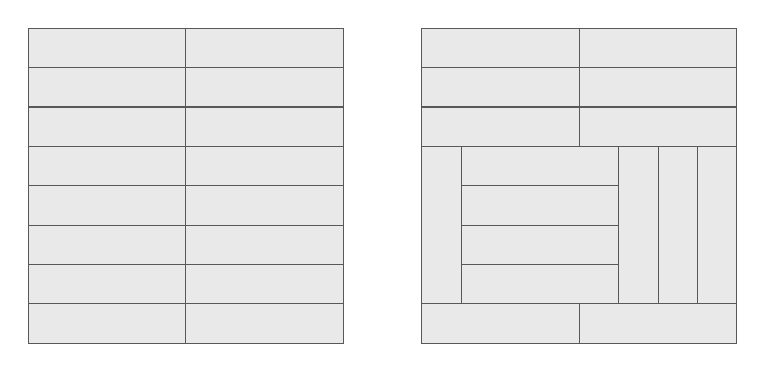
\begin{tikzpicture}[radius=0.1cm]
\selectcolormodel{cmyk}
\filldraw[fill=gray!20!white, draw=gray!50!black] (0,0) rectangle (2,0.5);
\filldraw[fill=gray!20!white, draw=gray!50!black] (2,0) rectangle (4,.5);
\filldraw[fill=gray!20!white, draw=gray!50!black] (0,.5) rectangle (4,1);
\filldraw[fill=gray!20!white, draw=gray!50!black] (2,.5) rectangle (4,1);
\filldraw[fill=gray!20!white, draw=gray!50!black] (0,1) rectangle (2,1.5);
\filldraw[fill=gray!20!white, draw=gray!50!black] (2,1) rectangle (4,1.5);
\filldraw[fill=gray!20!white, draw=gray!50!black] (0,1.5) rectangle (2,2);
\filldraw[fill=gray!20!white, draw=gray!50!black] (2,1.5) rectangle (4,2);

\filldraw[fill=gray!20!white, draw=gray!50!black] (0,2) rectangle (2,2.5);
\filldraw[fill=gray!20!white, draw=gray!50!black] (2,2) rectangle (4,2.5);
\filldraw[fill=gray!20!white, draw=gray!50!black] (0,2.5) rectangle (2,3);
\filldraw[fill=gray!20!white, draw=gray!50!black] (2,2.5) rectangle (4,3);
\filldraw[fill=gray!20!white, draw=gray!50!black] (0,3) rectangle (2,3.5);
\filldraw[fill=gray!20!white, draw=gray!50!black] (2,3) rectangle (4,3.5);
\filldraw[fill=gray!20!white, draw=gray!50!black] (0,3.5) rectangle (2,4);
\filldraw[fill=gray!20!white, draw=gray!50!black] (2,3.5) rectangle (4,4);

\filldraw[fill=gray!20!white, draw=gray!50!black] (5,0) rectangle (7,.5);
\filldraw[fill=gray!20!white, draw=gray!50!black] (7,0) rectangle (9,.5);

\filldraw[fill=gray!20!white, draw=gray!50!black] (5,.5) rectangle (5.5,2.5);
\filldraw[fill=gray!20!white, draw=gray!50!black] (5.5,.5) rectangle (7.5,1);
\filldraw[fill=gray!20!white, draw=gray!50!black] (5.5,1) rectangle (7.5,1.5);
\filldraw[fill=gray!20!white, draw=gray!50!black] (5.5,1.5) rectangle (7.5,2);
\filldraw[fill=gray!20!white, draw=gray!50!black] (5.5,2) rectangle (7.5,2.5);
\filldraw[fill=gray!20!white, draw=gray!50!black] (7.5,.5) rectangle (8,2.5);
\filldraw[fill=gray!20!white, draw=gray!50!black] (8,.5) rectangle (8.5,2.5);
\filldraw[fill=gray!20!white, draw=gray!50!black] (8.5,.5) rectangle (9,2.5);

\filldraw[fill=gray!20!white, draw=gray!50!black] (5,2.5) rectangle (7,3);
\filldraw[fill=gray!20!white, draw=gray!50!black] (7,2.5) rectangle (9,3);

\filldraw[fill=gray!20!white, draw=gray!50!black] (5,3) rectangle (7,3.5);
\filldraw[fill=gray!20!white, draw=gray!50!black] (7,3) rectangle (9,3.5);

\filldraw[fill=gray!20!white, draw=gray!50!black] (5,3.5) rectangle (7,4);
\filldraw[fill=gray!20!white, draw=gray!50!black] (7,3.5) rectangle (9,4);
\end{tikzpicture}
\end{center}
\begin{center}
pic(1)\ \ \ \ \ \ \ \ \ \ \ \ \ \ \ \ \ \ \ \ \ \ \ \ \ \ \ \ \ \ \ \ \ \ pic(2)
\end{center}
图1的矩阵
$$\begin{bmatrix}
1&5&12&16&19&23&26&30&33&37&44&48&51&55&58&62\\
2&6&9&13&20&24&27&31&34&38&41&45&52&56&59&63\\
3&7&10&14&17&21&28&32&35&39&42&46&49&53&60&64\\
4&8&11&15&18&22&25&29&36&40&43&47&50&54&57&61\\\end{bmatrix}$$
图2的矩阵
$$\begin{bmatrix}
1&5&33&12&19&26&37&30&23&16&44&48&51&55&58&62\\
2&6&9&13&20&27&34&38&31&24&41&45&52&56&59&63\\
3&7&17&10&21&28&35&14&39&32&42&46&49&53&60&64\\
4&8&25&11&18&29&36&22&15&40&43&47&50&54&57&61\\\end{bmatrix}$$

这里举例的两个角标矩阵是满足证明中的第一步的分组性质的。

通过计算机编程,可以验证定理中的部分结果如下:
$$1 \times4,det(A) = pfaffian(A)^{4} = 1^{4}=1$$
$$4 \times4,det(A) = pfaffian(A)^{4} = 2^{4}=16$$
$$5 \times4,det(A) = pfaffian(A)^{4} = 3^{4}=81$$
$$6 \times4,det(A) = pfaffian(A)^{4} = 4^{4}=256$$
$$7 \times4,det(A) = pfaffian(A)^{4} = 5^{4}=625$$
$$8 \times4,det(A) = pfaffian(A)^{4} = 7^{4}=2401$$
代码参考 ${IndexMatrix[5]}$

\begin{theorem}
将(\ref{1})中的$p_{i}<p_{j}<p_{k}<p_{l}$修改为$p_{i}\in$ (\ref{2}),$p_{j}\in$ (\ref{3}),$p_{k}\in$ (\ref{4}),$p_{l}\in$ (\ref{5}).
矩阵$A$的下角标写成列向量形式,除满足formal1,formal2,formal3,formal4的元素以外,其余都为0,并且滚动行元素得到的新的列向量对应元素只有符号上的差别,那么仍然有$$det(A)=pfaffian(A)^{4}$$
\end{theorem}
\begin{proof}
归纳法。
首先对于矩阵外维数为4的情形显然成立。
假设在$4(n-1)$时成立,下证$4n$成立,
首先证明左边矩阵中的下标元矩阵都可以分解成四个pfaffian形式。假设存在某个列中包含$(4n-3,4n)$间的元素也包含$(1,4(n-1))$间的元素,
那么将这其中包含$(4n-3,4n)$间的元素剔除掉剩下的元素按某个周期归位,那么这个列上被$(4n-3,4n)$间元素所占据位置的元素,恰好都在某个$\xi$
列上,将这些元素还原,即可得到完全属于$(1,4(n-1))$之间的元素构成的列,而$\xi$变换得到的$\xi^{'}$如果还有元素$a$属于$(1,4(n-1))$间的元素,那么
肯定存在某个$\eta$中有元素属于这个元素$a$所在的周期,并且$\eta$中$a$元素所在的行位置恰好缺少的是$a$,我们先将$\eta$变换成只包含$a$所在周期的元素和$(4n-3,4n)$周期的元素$\eta^{'}$,基于假设,这总是可以做到的,那么交互$a$和$\eta^{'}$对应的行位置,那么得到的$\xi^{''}$最多还有一个元素不属于$(4n-3,4n)$周期,
如果确实还有一个这样的元素,类似的进行操作得到$\xi^{'''}$就是所有都在$(4n-3,4n)$周期的列了。类似的我们可以对其它列,其中包含$(4n-3,4n)$间的元素也包含$(1,4(n-1))$ 间的元素进行操作,最终得到完全属于$(4n-3,4n)$周期的列,因为对于每个列来说,列元素只能是以4为周期的顺序向量列之间行元素与行元素的交叉变换,所以这不会与之前的操作存在冲突,最终我们得到了四个元素都属于$(4n-3,4n)$间的列,和余下的列,那么有假设结论显然对变换后的这样的排列可以分解成四个pfaffian形式的列。
而变换都是可逆的,所以对于原始形式一样可以分解成四个pfaffian形式的列。四个右边可以合并成一个左边是显然的。
符号相同的证明,对于左边矩阵中的下标元矩阵由原始的正则型变换通过行变换而来,而每次变换都引起一次逆序数。这对于最终分斥的pfaffian形式来说也同样引起一次符号的变换,所以符号相同。
\end{proof}
从结构上看,定理对内维数为2的情形,约化掉的那些包含奇轮换的元素,没能包含进来,这在推广上感觉有点不够完美,或许有更为广义的推广,但是遗憾作者做了一些尝试没能找到,这是一个更具挑战的问题,如果您感兴趣,可以尝试一下。
\sec{3 此类形式矩阵性质}

\begin{define}  双重维数矩阵的乘法
   $$[a_{ij}][b_{ijkl}]=[c_{ijkl}]$$
   $$c_{ijkl} = \Sigma_{\xi}^{n}a_{i\xi}b_{\xi jkl}$$
\end{define}

\begin{theorem}\   乘法定理

    $$det(A_{ij}B_{ijkl})=det(A_{ij})det(B_{ijkl})$$
\end{theorem}

\begin{proof}

法一:
\begin{align*}
det(C_{ijkl})&=\sum \limits_{\sigma\tau\gamma}sgn\sigma sgn\tau sgn\gamma c_{\sigma(1)\tau(1)\gamma(1)1} c_{\sigma(2)\tau(2)\gamma(2)2}\cdots c_{\sigma(n)\tau(n)\gamma(n)n}\\
&=\sum \limits_{\sigma\tau\gamma}sgn\sigma sgn\tau sgn\gamma \Sigma_{\xi}^{n}a_{\sigma(1)\xi}b_{\xi \tau(1)\gamma(1)1} \Sigma_{\xi}^{n}a_{\sigma(2)\xi}b_{\xi \tau(2)\gamma(2)2}\cdots \Sigma_{\xi}^{n}a_{\sigma(n)\xi}b_{\xi \tau(n)\gamma(n)n}\\
&=\sum \limits_{\tau\gamma}sgn\tau sgn\gamma(\sum \limits_{\sigma}sgn\sigma  \Sigma_{\xi}^{n}a_{\sigma(1)\xi}b_{\xi \tau(1)\gamma(1)1} \Sigma_{\xi}^{n}a_{\sigma(2)\xi}b_{\xi \tau(2)\gamma(2)2}\cdots \Sigma_{\xi}^{n}a_{\sigma(n)\xi}b_{\xi \tau(n)\gamma(n)n})\\
&=\sum \limits_{\tau\gamma}sgn\tau sgn\gamma(det(A_{ij})\sum \limits_{\sigma}sgn\sigma b_{\sigma(1) \tau(1)\gamma(1)1} b_{\sigma(2) \tau(2)\gamma(2)1} \cdots b_{\sigma(n) \tau(n)\gamma(n)n})\\
&=det(A_{ij})det(B_{ijkl})
\end{align*}

法二:用外积来证明.

令

\begin{equation}
\begin{aligned}
\omega_{i}
&= \sum_{j_{\sigma}=1}^{n}\sum_{k_{\sigma}=1}^{n}\sum_{l_{\sigma}=1}^{n}b_{ij_{\sigma}k_{\sigma}l_{\sigma}} f_{1}^{j_{\sigma}} \wedge f_{2}^{k_{\sigma}} \wedge f_{3}^{l_{\sigma}}
\end{aligned}
\end{equation}

做基底变换如下:
$$(f_{1}^{1},f_{1}^{2},...,f_{1}^{n})=(e_{1}^{1},e_{1}^{2},...,e_{1}^{n})X_{1}$$
$$(f_{2}^{1},f_{2}^{2},...,f_{2}^{n})=(e_{2}^{1},e_{2}^{2},...,e_{2}^{n})X_{2}$$
$$(f_{3}^{1},f_{3}^{2},...,f_{3}^{n})=(e_{3}^{1},e_{3}^{2},...,e_{3}^{n})X_{3}$$
则
\begin{equation}
f_{1}^{j_{\sigma}}\wedge f_{2}^{k_{\sigma}}\wedge f_{3}^{l_{\sigma}}
\begin{aligned}
& = \sum_{\xi_{1}=1}^{n}\sum_{\xi_{2}=1}^{n}\sum_{\xi_{3}=1}^{n}x_{1}^{\xi_{1}j_{\sigma}}x_{2}^{\xi_{2}k_{\sigma}}x_{3}^{\xi_{
3}l_{\sigma}}e_{1}^{\xi_{1}}\wedge e_{2}^{\xi_{2}}\wedge e_{3}^{\xi_{3}}
\end{aligned}
\end{equation}

从而,
\begin{equation}
\begin{aligned}
\omega_{i}
&= \sum_{j_{\sigma}=1}^{n}\sum_{k_{\sigma}=1}^{n}\sum_{l_{\sigma}=1}^{n} b_{ij_{\sigma}k_{\sigma}l_{\sigma}} f_{1}^{j_{\sigma}} \wedge f_{2}^{k_{\sigma}} \wedge f_{3}^{l_{\sigma}} \\
&= \sum_{j_{\sigma}=1}^{n}\sum_{k_{\sigma}=1}^{n}\sum_{l_{\sigma}=1}^{n} b_{ij_{\sigma}k_{\sigma}l_{\sigma}}
\sum_{\xi_{1}=1}^{n}\sum_{\xi_{2}=1}^{n}\sum_{\xi_{3}=1}^{n}x_{1}^{\xi_{1}j_{\sigma}}x_{2}^{\xi_{2}k_{\sigma}}x_{3}^{\xi_{3}l_{\sigma}}e_{1}^{\xi_{1}}\wedge e_{2}^{\xi_{2}}\wedge e_{3}^{\xi_{3}}\\
&= \sum_{\xi_{1}=1}^{n}\sum_{\xi_{2}=1}^{n}\sum_{\xi_{3}=1}^{n}\sum_{j_{\sigma}=1}^{n}\sum_{k_{\sigma}=1}^{n}\sum_{l_{\sigma}=1}^{n}b_{ij_{\sigma}k_{\sigma}l_{\sigma}}
x_{1}^{\xi_{1}j_{\sigma}}x_{2}^{\xi_{2}k_{\sigma}}x_{3}^{\xi_{3}l_{\sigma}}e_{1}^{\xi_{1}}\wedge e_{2}^{\xi_{2}}\wedge e_{3}^{\xi_{3}}
\end{aligned}\end{equation}
从而得到
$$a_{ijkl}=\sum_{j_{\sigma}=1}^{n}\sum_{k_{\sigma}=1}^{n}\sum_{l_{\sigma}=1}^{n}b_{ij_{\sigma}k_{\sigma}l_{\sigma}}x_{1}^{jj_{\sigma}}x_{2}^{kk_{\sigma}}x_{3}^{ll_{\sigma}}$$
由前述定理得到
\begin{equation}
\begin{aligned}
\omega_{1}\wedge\omega_{2}\wedge\cdots\wedge\omega_{n}
& = det(B) f_{1}^1\wedge f_{1}^2 \cdots \wedge f_{1}^n \wedge f_{2}^1\wedge f_{2}^2 \cdots \wedge f_{2}^n
\wedge f_{3}^1\wedge f_{3}^2 \cdots \wedge f_{3}^n\\
& = det(B)det(X_{1})det(X_{2})det(X_{3}) \\
&e_{1}^1\wedge e_{1}^2 \cdots \wedge e_{1}^n \wedge e_{2}^1\wedge e_{2}^2 \cdots \wedge e_{2}^n
\wedge e_{3}^1\wedge e_{3}^2 \cdots \wedge e_{3}^n\\
\end{aligned}
\end{equation}
即证 $det(A) = det(B)det(X_{1})det(X_{2})det(X_{3})$
\\
\end{proof}

\begin{theorem}  $A_{ijkl}$的拉普拉斯定理
$$det(A)=\sum\limits_{j=1}^n \sum\limits_{k=1}^n \sum\limits_{l=1}^n (-1)^{i+j+k+l} a_{i,j,k,l} A^{*}_{i,j,k,l} $$
\end{theorem}
\begin{proof}
左边单项都属于右边且符号相同,项数也是相同的,结果是显而易见的。
\end{proof}

推广的命题是,
$$detA=\sum\limits_{j_{1}j_{2}...j_{p}} \sum\limits_{k_{1}k_{2}...k_{p}} \sum\limits_{l_{1}l_{2}...l_{p}}
(-1)^{\sum_{t=1}^{p}(i_{t}+j_{t}+k_{t}+l_{t})}
M_{\left(\begin{array}{cccc}
i_{1} & i_{2} & \cdots & i_{p} \\
j_{1} & j_{2} & \cdots & j_{p} \\
k_{1} & k_{2} & \cdots & k_{p} \\
l_{1} & l_{2} & \cdots & l_{p} \\
\end{array}\right)}
A^{*}_{\left(\begin{array}{cccc}
i_{p+1} & i_{p+2} & \cdots & i_{n} \\
j_{p+1} & j_{p+2} & \cdots & j_{n} \\
k_{p+1} & k_{p+2} & \cdots & k_{n} \\
l_{p+1} & l_{p+2} & \cdots & l_{n} \\
\end{array}\right)}$$
项数上的关系是左边$(n!)^{3}$,右边是$(\frac{(n!)^{3}}{(p!(n-p)!))^{3}})(p!)^{3}[(n-p)!]^{3}$结论也比较显然。

\begin{define}
矩阵的克罗内克积
\\
   $$\begin{bmatrix}\begin{smallmatrix}
  A_{11}& A_{12}& \cdots&A_{1n}\\
  A_{21}& A_{22}& \cdots&A_{2n}\\
  & & \cdots&\\&\\
  A_{n1}& A_{n2}& \cdots&A_{nn}\\
 \end{smallmatrix}\end{bmatrix}
 \times
 \begin{bmatrix}\begin{smallmatrix}
  B_{11}& B_{12}& \cdots&B_{1m}\\
  B_{21}& B_{22}& \cdots&B_{2m}\\
  & & \cdots&\\&\\
  B_{m1}& B_{m2}& \cdots&B_{mm}\\
 \end{smallmatrix}\end{bmatrix}\\$$
 $$=\\
 \begin{bmatrix}\begin{smallmatrix}
  A_{11} \times B_{11}& A_{12} \times B_{11}& \cdots&A_{1n} \times B_{11}
  & & \cdots&
  A_{11} \times B_{1m}& A_{12} \times B_{1m}& \cdots&A_{1n} \times B_{1m}\\
  A_{21} \times B_{11}& A_{22} \times B_{11}& \cdots&A_{2n} \times B_{11}
  & & \cdots&
  A_{21} \times B_{1m}& A_{22} \times B_{1m}& \cdots&A_{2n} \times B_{1m}\\
  & & & & &\cdots& &\\
  A_{n1} \times B_{11}& A_{n2} \times B_{11}& \cdots&A_{nn} \times B_{11}
  & & \cdots&
  A_{n1} \times B_{1m}& A_{n2} \times B_{1m}& \cdots&A_{nn} \times B_{1m}\\
  \cdots &\cdots &\cdots &\cdots &\cdots  &\cdots  &\cdots &\cdots  &\cdots &\cdots \\
  A_{11} \times B_{m1}& A_{12} \times B_{m1}& \cdots&A_{1n} \times B_{m1}
  & & \cdots&
  A_{11} \times B_{mm}& A_{12} \times B_{mm}& \cdots&A_{1n} \times B_{mm}\\
  A_{21} \times B_{m1}& A_{22} \times B_{m1}& \cdots&A_{2n} \times B_{m1}
  & & \cdots&
  A_{21} \times B_{mm}& A_{22} \times B_{mm}& \cdots&A_{2n} \times B_{mm}\\
  & & & & &\cdots& &\\
  A_{n1} \times B_{m1}& A_{n2} \times B_{m1}& \cdots&A_{nn} \times B_{m1}
  & & \cdots&
  A_{n1} \times B_{mm}& A_{n2} \times B_{mm}& \cdots&A_{nn} \times B_{mm}\\
  \end{smallmatrix}\end{bmatrix}$$
\end{define}

\sec{4 计算}
类似 Kasteleyn$^{[1]}$中将计算的矩阵表达成
$D=z(Q_{n}\times E_{m})  +  z^{'} (F_{n} \times Q_{m})$
由上面的定义,这里关于$tetramer$的计算也可以表达成两个类型的和式。
假设矩形方块为$n\times m$,
$$
  Q_{n} = \begin{bmatrix}\begin{smallmatrix}
  0& 0&
  \begin{bmatrix}\begin{smallmatrix}
 0& 0& 0&0&0&\cdots&0\\
 0& 0& 0&1&0&\cdots&0\\
 0& 0& 0&0&0&\cdots&0\\
 0& 0& 0&0&0&\cdots&0\\
 0& 0& 0&0&0&\cdots&0\\
 & & \cdots& &\\
0& 0&0& 0&\cdots&0\\
 \end{smallmatrix}\end{bmatrix}& 0& 0& 0& \cdots&\\
 0& 0& 0&
   \begin{bmatrix}\begin{smallmatrix}
 0& 0& 0&0&0&\cdots&0\\
 0& 0& 0&0&0&\cdots&0\\
 1& 0& 0&0&1&\cdots&0\\
 0& 0& 0&0&0&\cdots&0\\
 0& 0& 0&0&0&\cdots&0\\
 & & \cdots& &\\
0& 0&0& 0&0&\cdots&0\\
 \end{smallmatrix}\end{bmatrix}&0& 0&\cdots\\
 \begin{bmatrix}\begin{smallmatrix}
 0& 0& 0&0&0&\cdots&0\\
 0& 0& 0&0&0&\cdots&0\\
 0& 0& 0&0&0&\cdots&0\\
 0& 1& 0&0&0&\cdots&0\\
 0& 0& 0&0&0&\cdots&0\\
 & & \cdots& &\\
0& 0& 0& 0&0&\cdots&0\\
 \end{smallmatrix}\end{bmatrix}&
 0& 0& 0&
 \begin{bmatrix}\begin{smallmatrix}
 0& 0& 0&0&0&\cdots&0\\
 0& 0& 0&0&0&\cdots&0\\
 0& 0& 0&0&0&\cdots&0\\
 0& 1& 0&0&0&\cdots&0\\
 0& 0& 0&0&0&\cdots&0\\
 & & \cdots& &\\
0& 0& 0& 0&0&\cdots&0\\
 \end{smallmatrix}\end{bmatrix}&
 0& \cdots&\\
 0& \begin{bmatrix}\begin{smallmatrix}
  0& 0& 1&0&0&\cdots&0\\
 0& 0& 0&0&0&\cdots&0\\
 0& 0& 0&0&0&\cdots&0\\
 0& 0& 0&0&0&\cdots&0\\
 0& 0& 1&0&0&\cdots&0\\
 & & \cdots& &\\
0& 0& 0& 0&0&\cdots&0\\
 \end{smallmatrix}\end{bmatrix}& 0& 0& 0&
 \begin{bmatrix}\begin{smallmatrix}
  0& 0& 0&0&0&\cdots&0\\
 0& 0& 0&0&0&\cdots&0\\
 0& 0& 0&0&0&\cdots&0\\
 0& 0& 0&0&0&\cdots&0\\
 0& 0& 1&0&0&\cdots&0\\
 & & \cdots& &\\
0& 0& 0& 0&0&\cdots&0\\
 \end{smallmatrix}\end{bmatrix}& \cdots&\\
 0& 0& \ddots &0 &0 &0 &\ddots \\
\end{smallmatrix}\end{bmatrix}$$

$$= \begin{bmatrix}\begin{smallmatrix}
 0& 0& A^{1}_{n} & 0 &\cdots& 0\\
  0& 0& 0 & A^{2}_{n} &\cdots& 0\\
 A^{1T}_{n} & 0& 0 & 0 &\cdots& 0\\
 0& A^{2T}_{n} & 0 & 0 &\cdots& 0\\
 & & \cdots & &\\
\end{smallmatrix}\end{bmatrix}_{n} $$
$Q_{n}\times E_{m}$
那么有结果
$D=z(Q_{n}\times E_{m})  +  z^{'} (E_{n} \times Q_{m})$。\\
\sec{5 展望}
在内维数为2的情形,特征值和特征向量是研究矩阵非常有用的工具,在内维数为4的情形如何展开研究?
显然,仍可以通过$det(\lambda E - A) = 0$求出特征值,并满足这些特征值的乘积恰好等于$det(A)$。但是对任意的可逆矩阵却没有相似变换保证对$E$做完变换后保持不变。什么样的变换能保证$E$不变?什么样的矩阵可以通过类似内维数为2的情况进行相似变换后对角化?这些问题很值得研究。

 \sec{参考文献}
\baselineskip 13pt {\footnotesize

\REF{[1]} P. W. Kasteleyn, The statistics of dimers on a lattice, {\it Physica.}, 1961, 27.

\REF{[2]} Richard Kenyon, Andrei Okounkov,  What is ... a dimer?, {\it Notices of the American Mathematical Society} MARCH 2005 VOLUME 52, NUMBER 3.

\REF{[3]} https://github.com/huih1984/tetramerVc/blob/master/IndexMatrix.cpp%<link  href="https://github.com/huih1984/tetramerVc/blob/master/IndexMatrix.cpp">
\REF{[4]} RICHARD J. MATHAR PAVING RECTANGULAR REGIONS WITH RECTANGULAR TILES: TATAMI AND NON-TATAMI TILINGS.{\it arXiv:1311.6135v1 [math.CO]},  24 Nov 2013
\vskip .25in

\centerline{\Large  The statistics of tetramers on a lattice }\vskip
.1in

\centerline{\normalsize\zihao{5} Hui Hui$^{1}$}\vskip .13in

{\small({\it  1. Department of Mathematics, NanJing University, Nanjing,
Jiangsu, 210093, P. R. China})}\vskip .23in

\baselineskip 14pt \zihao{5}\normalsize {\indent{\bf Abstract:}\ \
The article Kasteleyn$^{[1]}$ transfer dimer tiling to determinant of matrix ingenious, finally, get formula of it.
so, what about of three,four?this is intreseting.\\
{\bf Key words:double dimension matrix; inner dimension; domino tiling; wedge product; pfaffian;trimer; dimer; tertramer}\ \

}
\end{document}
